\documentclass[../main.tex]{subfiles}
\begin{document}

\theoremstyle{definition}

\chapter{LU Factorization}

\begin{center}
\textbf{CHAPTER OBJECTIVES}
\end{center}
The primary objective of this chapter is to acquaint you with \textit{LU} factorization.\label{oneLU}\footnote{In the parlance of numerical methods, the terms “factorization” and “decomposition” are synonymous. To be
consistent with the MATLAB documentation, we have chosen to employ the terminology LU factorization for
the subject of this chapter. Note that LU decomposition is very commonly used to describe the same approach.}
Specific objectives and topics covered are
\begin{itemize}
	\item Understanding that \textit{LU} factorization involves decomposing the coefficient matrix into two triangular matrices that can then be used to efficiently evaluate different right-hand-side vectors.
	\item Knowing how to express Gauss elimination as an \textit{LU} factorization.
	\item Given an \textit{LU} factorization, knowing how to evaluate multiple right-hand-side vectors.
	\item Recognizing that Cholesky’s method provides an efficient way to decompose a symmetric matrix and that the resulting triangular matrix and its transpose can be used to evaluate right-hand-side vectors efficiently.
	\item Understanding in general terms what happens when MATLAB’s backslash operator is used to solve linear systems.
\end{itemize}

As described in Chap. 9, Gauss elimination is designed to solve systems of linear algebraic equations:
$$[A]{x}={b}$$
\begin{flushright}
(10.1)
\end{flushright}
Although it certainly represents a sound way to solve such systems, it becomes inefficient when solving equations with the same coefficients $[A]$, but with different right-hand-side constants $\{b\}$.

Recall that Gauss elimination involves two steps: forward elimination and back substitution (Fig. 9.3). As we learned in Section 9.2.2, the forward-elimination step comprises the bulk of the computational effort. This is particularly true for large systems of equations.

$LU$ factorization methods separate the time-consuming elimination of the matrix $[A]$ from the manipulations of the right-hand side $\{b\}$. Thus, once $[A]$ has been "factored" or "decomposed," multiple right-hand-side vectors can be evaluated in an efficient manner.

Interestingly, Gauss elimination itself can be expressed as an $LU$ factorization. Before showing how this can be done, let us first provide a mathematical overview of the factorization strategy.

\section{OVERVIEW OF LU FACTORIZATION}

Just as was the case with Gauss elimination, $LU$ factorization requires pivoting to avoid division by zero. However, to simplify the following description, we will omit pivoting. In addition, the following explanation is limited to a set of three simultaneous equations. The results can be directly extended to $n$-dimensional systems.

Equation (10.1) can be rearranged to give

\begin{equation}
[A]\{x\}-\{b\}=0\tag{10.2}
\end{equation}
Suppose that Eq. (10.2) could be expressed as an upper triangular system. For example, for a $3 \times 3$ system:
\begin{equation}
\begin{bmatrix}
u_{11} &u_{12}  &u_{13} \\
0 &u_{22}  &u_{23} \\
0 &0  &u_{33}
\end{bmatrix}
\begin{Bmatrix}
x_{1}\\
x_{2}\\
x_{3}
\end{Bmatrix}=
\begin{Bmatrix}
d_{1}\\
d_{2}\\
d_{3}
\end{Bmatrix}\tag{10.3}
\end{equation}
Recognize that this is similar to the manipulation that occurs in the first step of Gauss elimination. That is, elimination is used to reduce the system to upper triangular form. Equation (10.3) can also be expressed in matrix notation and rearranged to give
\begin{equation}
[U]\{x\}-\{d\}=0\tag{10.4}
\end{equation}
Now assume that there is a lower diagonal matrix with 1’s on the diagonal,
\begin{equation}
[L]=
\begin{bmatrix}
1 &0  &0 \\
l_{21} &1  &0 \\
l_{31} &l_{32}  &1
\end{bmatrix}\tag{10.5}
\end{equation}
that has the property that when Eq. (10.4) is premultiplied by it, Eq. (10.2) is the result. That is,
\begin{equation}
[L]\{[U]\{x\}-\{d\}\}=[A]\{x\}-\{b\}\tag{10.6}
\end{equation}
If this equation holds, it follows from the rules for matrix multiplication that
\begin{equation}
[L][U]=[A]\tag{10.7}
\end{equation}
and
\begin{equation}
[L]\{d\}=\{b\}\tag{10.8}
\end{equation}

\begin{figure}[H]
	\centering
	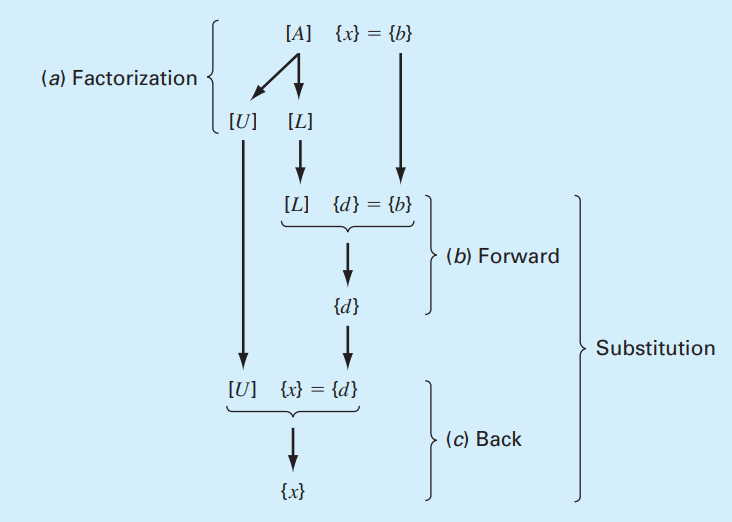
\includegraphics[width=0.75\textwidth]{fig_10_15}
	\caption{\textsf{The steps in LU factorization.}}
	\label{fig:fig_10_15}
\end{figure}

A two-step strategy (see Fig. 10.1) for obtaining solutions can be based on Eqs. (10.3), (10.7), and (10.8):

\begin{enumerate}
\item LU factorization step. [A] is factored or “decomposed” into lower [L] and upper [U] triangular matrices.
\item Substitution step. [L] and [U] are used to determine a solution {x} for a right-hand side $\{b\}$ . This step itself consists of two steps. First, Eq. (10.8) is used to generate an intermediate vector $\{d\}$ by forward substitution. Then, the result is substituted into Eq. (10.3) which can be solved by back substitution for $\{x\}$.
\end{enumerate}
Now let us show how Gauss elimination can be implemented in this way.

\section{GAUSS ELIMINATION AS LU FACTORIZATION}

Although it might appear at face value to be unrelated to LU factorization, Gauss elimination can be used to decompose [A] into [L] and [U]. This can be easily seen for [U], which is a direct product of the forward elimination. Recall that the forward-elimination step is intended to reduce the original coefficient matrix [A] to the form
\begin{equation}
[U]=
\begin{bmatrix}
a_{11} &a_{12}  &a_{13} \\
0 &a'_{22}  &a'_{23} \\
0 &0  &a''_{33}
\end{bmatrix}\tag{10.9}
\end{equation}
which is in the desired upper triangular format.

Though it might not be as apparent, the matrix [L] is also produced during the step. This can be readily illustrated for a three-equation system,
\begin{equation}
\begin{bmatrix}
a_{11} &a_{12}  &a_{13} \\
a_{21} &a_{22}  &a_{23} \\
a_{31} &a_{32}  &a_{33}
\end{bmatrix}
\begin{Bmatrix}
x_{1}\\
x_{2}\\
x_{3}
\end{Bmatrix}=
\begin{Bmatrix}
b_{1}\\
b_{2}\\
b_{3}
\end{Bmatrix}
\end{equation}
The first step in Gauss elimination is to multiply row 1 by the factor [recall Eq. (9.9)]
\begin{equation}
f_{21}=\frac{a_{21}}{a_{11}}
\end{equation}
and subtract the result from the second row to eliminate $a_{21}$. Similarly, row 1 is multiplied by
\begin{equation}
f_{31}=\frac{a_{31}}{a_{11}}
\end{equation}
and the result subtracted from the third row to eliminate $a_{31}$. The final step is to multiply the modified second row by
\begin{equation}
f_{32}=\frac{a'_{32}}{a'_{22}}
\end{equation}
and subtract the result from the third row to eliminate $a'_{32}$.

Now suppose that we merely perform all these manipulations on the matrix [A]. Clearly, if we do not want to change the equations, we also have to do the same to the righthand side $\{b\}$. But there is absolutely no reason that we have to perform the manipulations simultaneously. Thus, we could save the f’s and manipulate $\{b\}$ later

Where do we store the factors $f_{21}$, $f_{31}$, and $f_{32}$? Recall that the whole idea behind the elimination was to create zeros in $a_{21}$, $a_{31}$, and $a_{32}$. Thus, we can store $f_{21}$ in $a_{21}$, $f_{31}$ in $a_{31}$, and $f_{32}$ in $a_{32}$. After elimination, the [A] matrix can therefore be written as
\begin{equation}
\begin{bmatrix}
a_{11} &a_{12}  &a_{13} \\
f_{21} &a'_{22}  &a'_{23} \\
f_{31} &f_{32}  &a''_{33}
\end{bmatrix}\tag{10.10}
\end{equation}
This matrix, in fact, represents an efficient storage of the LU factorization of [A],
\begin{equation}
[A]\rightarrow [L][U]\tag{10.11}
\end{equation}
where
\begin{equation}
\begin{bmatrix}
a_{11} &a_{12}  &a_{13} \\
0 &a'_{22}  &a'_{23} \\
0 &0  &a''_{33}
\end{bmatrix}\tag{10.12}
\end{equation}
and
\begin{equation}
\begin{bmatrix}
1 &0  &0 \\
f_{21} &1  &0 \\
f_{31} &f_{32}  &1
\end{bmatrix}\tag{10.13}
\end{equation}
The following example confirms that $[A]=[L][U]$.

\section*{EXAMPLE 10.1 LU Factorization with Gauss Elimination}

Problem Statement. Derive an LU factorization based on the Gauss elimination performed previously in Example 9.3.
Solution. In Example 9.3, we used Gauss elimination to solve a set of linear algebraic equations that had the following coefficient matrix:
\begin{equation}
[A]=\begin{bmatrix}
3 &-0.1  &-0.2 \\
0.1 &7  &-0.3 \\
0.3 &-0.2  & 10
\end{bmatrix}
\end{equation}
After forward elimination, the following upper triangular matrix was obtained:
\begin{equation}
[U]=\begin{bmatrix}
3 &-0.1  &-0.2 \\
0 &7.00333  &-0.293333 \\
0 &0  & 10.0120
\end{bmatrix}
\end{equation}
The factors employed to obtain the upper triangular matrix can be assembled into a lower triangular matrix. The elements a21 and a31 were eliminated by using the factors
\begin{equation}
f_{21}=\frac{0.1}{3}=0.0333333
\; \; \; \; \; \;
f_{31}=\frac{0.3}{3}=0.1000000
\end{equation}
and the element $a_{32}$ was eliminated by using the factor
\begin{equation}
f_{32}=\frac{-0.19}{7.00333}=-0.0271300
\end{equation}
Thus, the lower triangular matrix is
\begin{equation}
[L]=\begin{bmatrix}
1 &0  &0 \\
0.0333333 &1  &0 \\
0.100000 &0.0271300   & 1
\end{bmatrix}
\end{equation}
Consequently, the LU factorization is
\begin{equation}
[A]=[L][U]=\begin{bmatrix}
1 &0  &0 \\
0.0333333 &1  &0 \\
0.100000 &0.0271300   & 1
\end{bmatrix}
\begin{bmatrix}
3 &-0.1  &-0.2 \\
0 &7.00333  &-0.293333 \\
0 &0  & 10.0120
\end{bmatrix}
\end{equation}
This result can be verified by performing the multiplication of [L][U] to give
\begin{equation}
[L][U]=
\begin{bmatrix}
3 &-0.1  &-0.2 \\
0.0999999 &7  &-0.3 \\
0.3 &-0.2  & 9.99996
\end{bmatrix}
\end{equation}
where the minor discrepancies are due to roundoff.

After the matrix is decomposed, a solution can be generated for a particular right-handside vector $\{b\}$. This is done in two steps. First, a forward-substitution step is executed by solving Eq. (10.8) for $\{d\}$. It is important to recognize that this merely amounts to performing the elimination manipulations on $\{b\}$. Thus, at the end of this step, the right-hand side
will be in the same state that it would have been had we performed forward manipulation on [A] and $\{b\}$ simultaneously.

The forward-substitution step can be represented concisely as
\begin{equation}
d_{i}=b_{i}-\sum^{i-1}_{j=1}l_{ij}d_{j}
\; \; \; \; \; \;
for\; \; i=n-1,n-2,\cdots,1
\end{equation}

The second step then merely amounts to implementing back substitution to solve
Eq. (10.3). Again, it is important to recognize that this is identical to the back-substitution phase of conventional Gauss elimination [compare with Eqs. (9.12) and (9.13)]:
\begin{equation}
x_{n}=d_{n}/u_{nn}
\end{equation}
\begin{equation}
x_{i}=\frac{d_{i}-\sum^{n}_{j=i+1}u_{ij}x_{j}}{u{ii}}
\; \; \; \; \; \;
for\; \; i=n-1,n-2,\cdots,1
\end{equation}

\end{document}



% 279 TODO
